\subsection{Main Page}
In this page as shown in figure \ref{fig:user-main}, the user can 

\begin{enumerate}
    \item choose from a menu the generation mode that he or she wants.
    \item navigate to the demo and help page from the bar in the header.
\end{enumerate}
    
\begin{figure}[H]
    \centering
    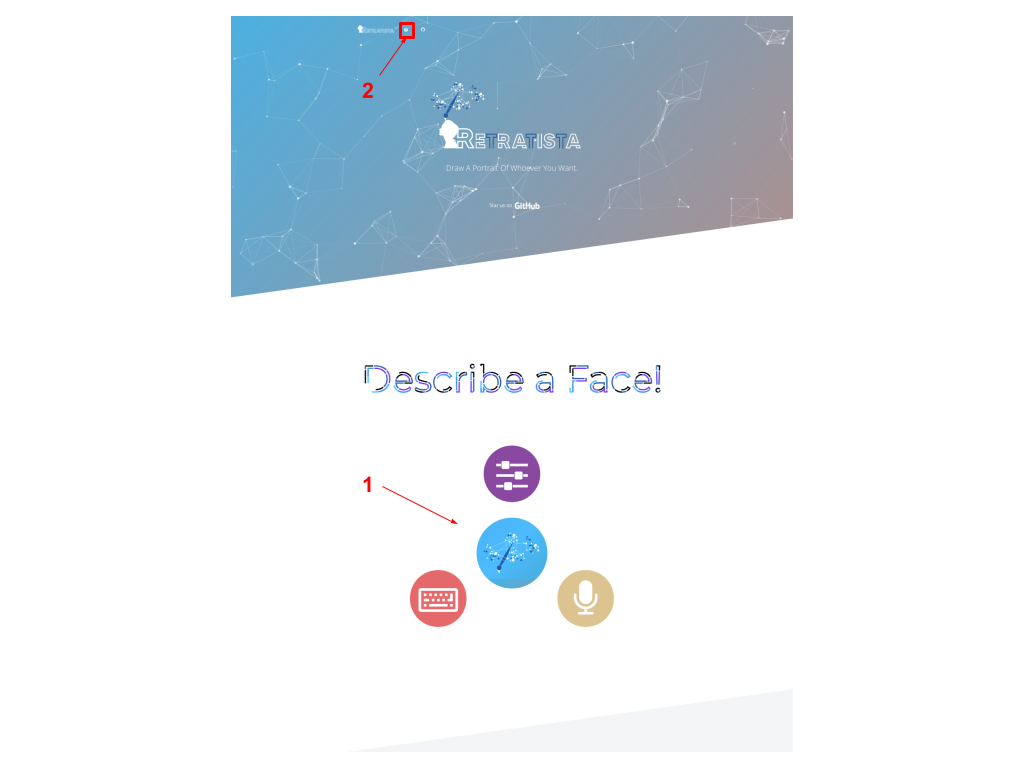
\includegraphics[width=1.0\textwidth]{images/guide/main.png}
    \caption{Main Page}
    \label{fig:user-main}
\end{figure}


\subsection{Voice Description Page}
In this page as shown in figure \ref{fig:user-voice}, the user can 

\begin{enumerate}
    \item describe a face using his voice.
    \item edit the description textually.
    \item generate the described face.
    \item route to refine page after generation.
    \item route to head poses page after generation.
\end{enumerate}

\begin{figure}[H]
    \centering
    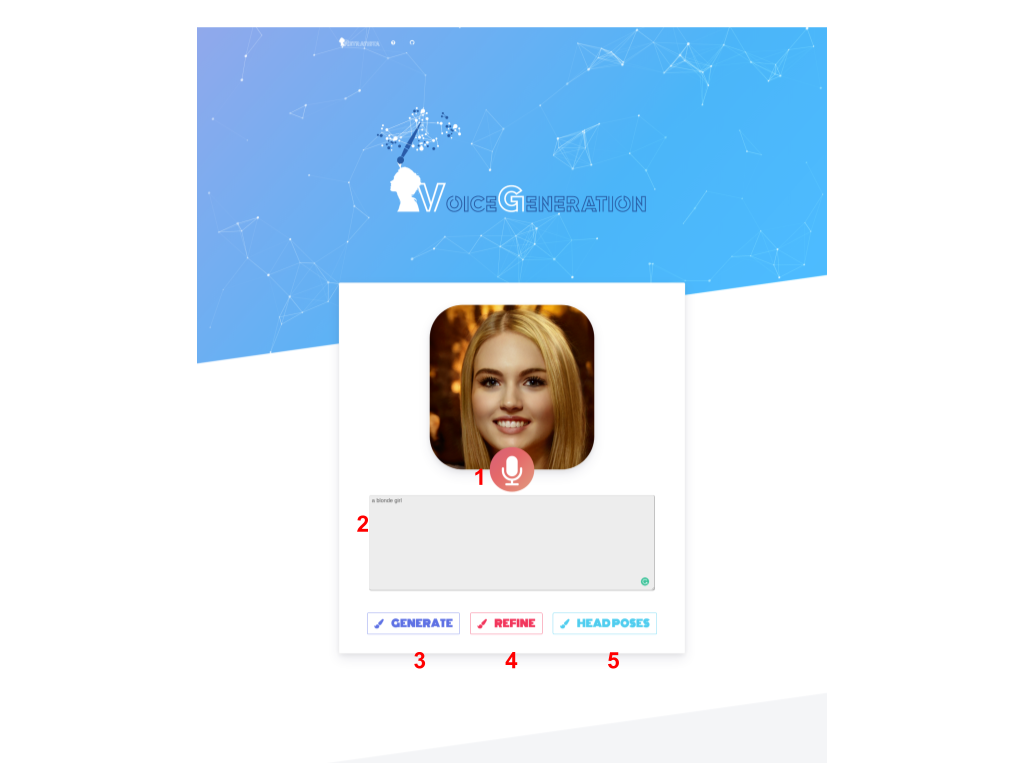
\includegraphics[width=1.0\textwidth]{images/guide/voice.png}
    \caption{Voice Description Page}
    \label{fig:user-voice}
\end{figure}


\subsection{Text Description Page}
In this page as shown in figure \ref{fig:user-text}, the user can 

\begin{enumerate}
    \item describe a face textually.
    \item generate the described face.
    \item route to refine page after generation.
    \item route to head poses page after generation.
\end{enumerate}

\begin{figure}[H]
    \centering
    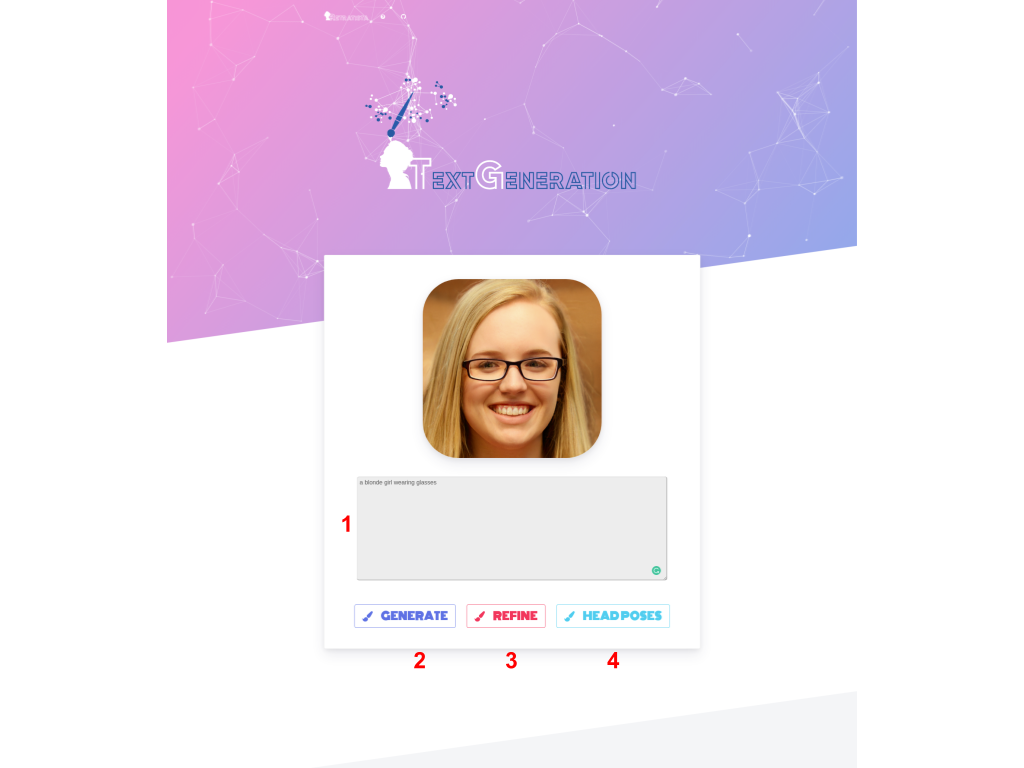
\includegraphics[width=1.0\textwidth]{images/guide/text.png}
    \caption{Text Description Page}
    \label{fig:user-text}
\end{figure}


\subsection{Refine Page}
In this page as shown in figure \ref{fig:user-refine} for refinement of age attribute, the user can 

\begin{enumerate}
    \item navigate in 39 different facial attributes to get the actual intended face.
    \item route to head poses page after refinement.
\end{enumerate}

\begin{figure}[H]
    \centering
    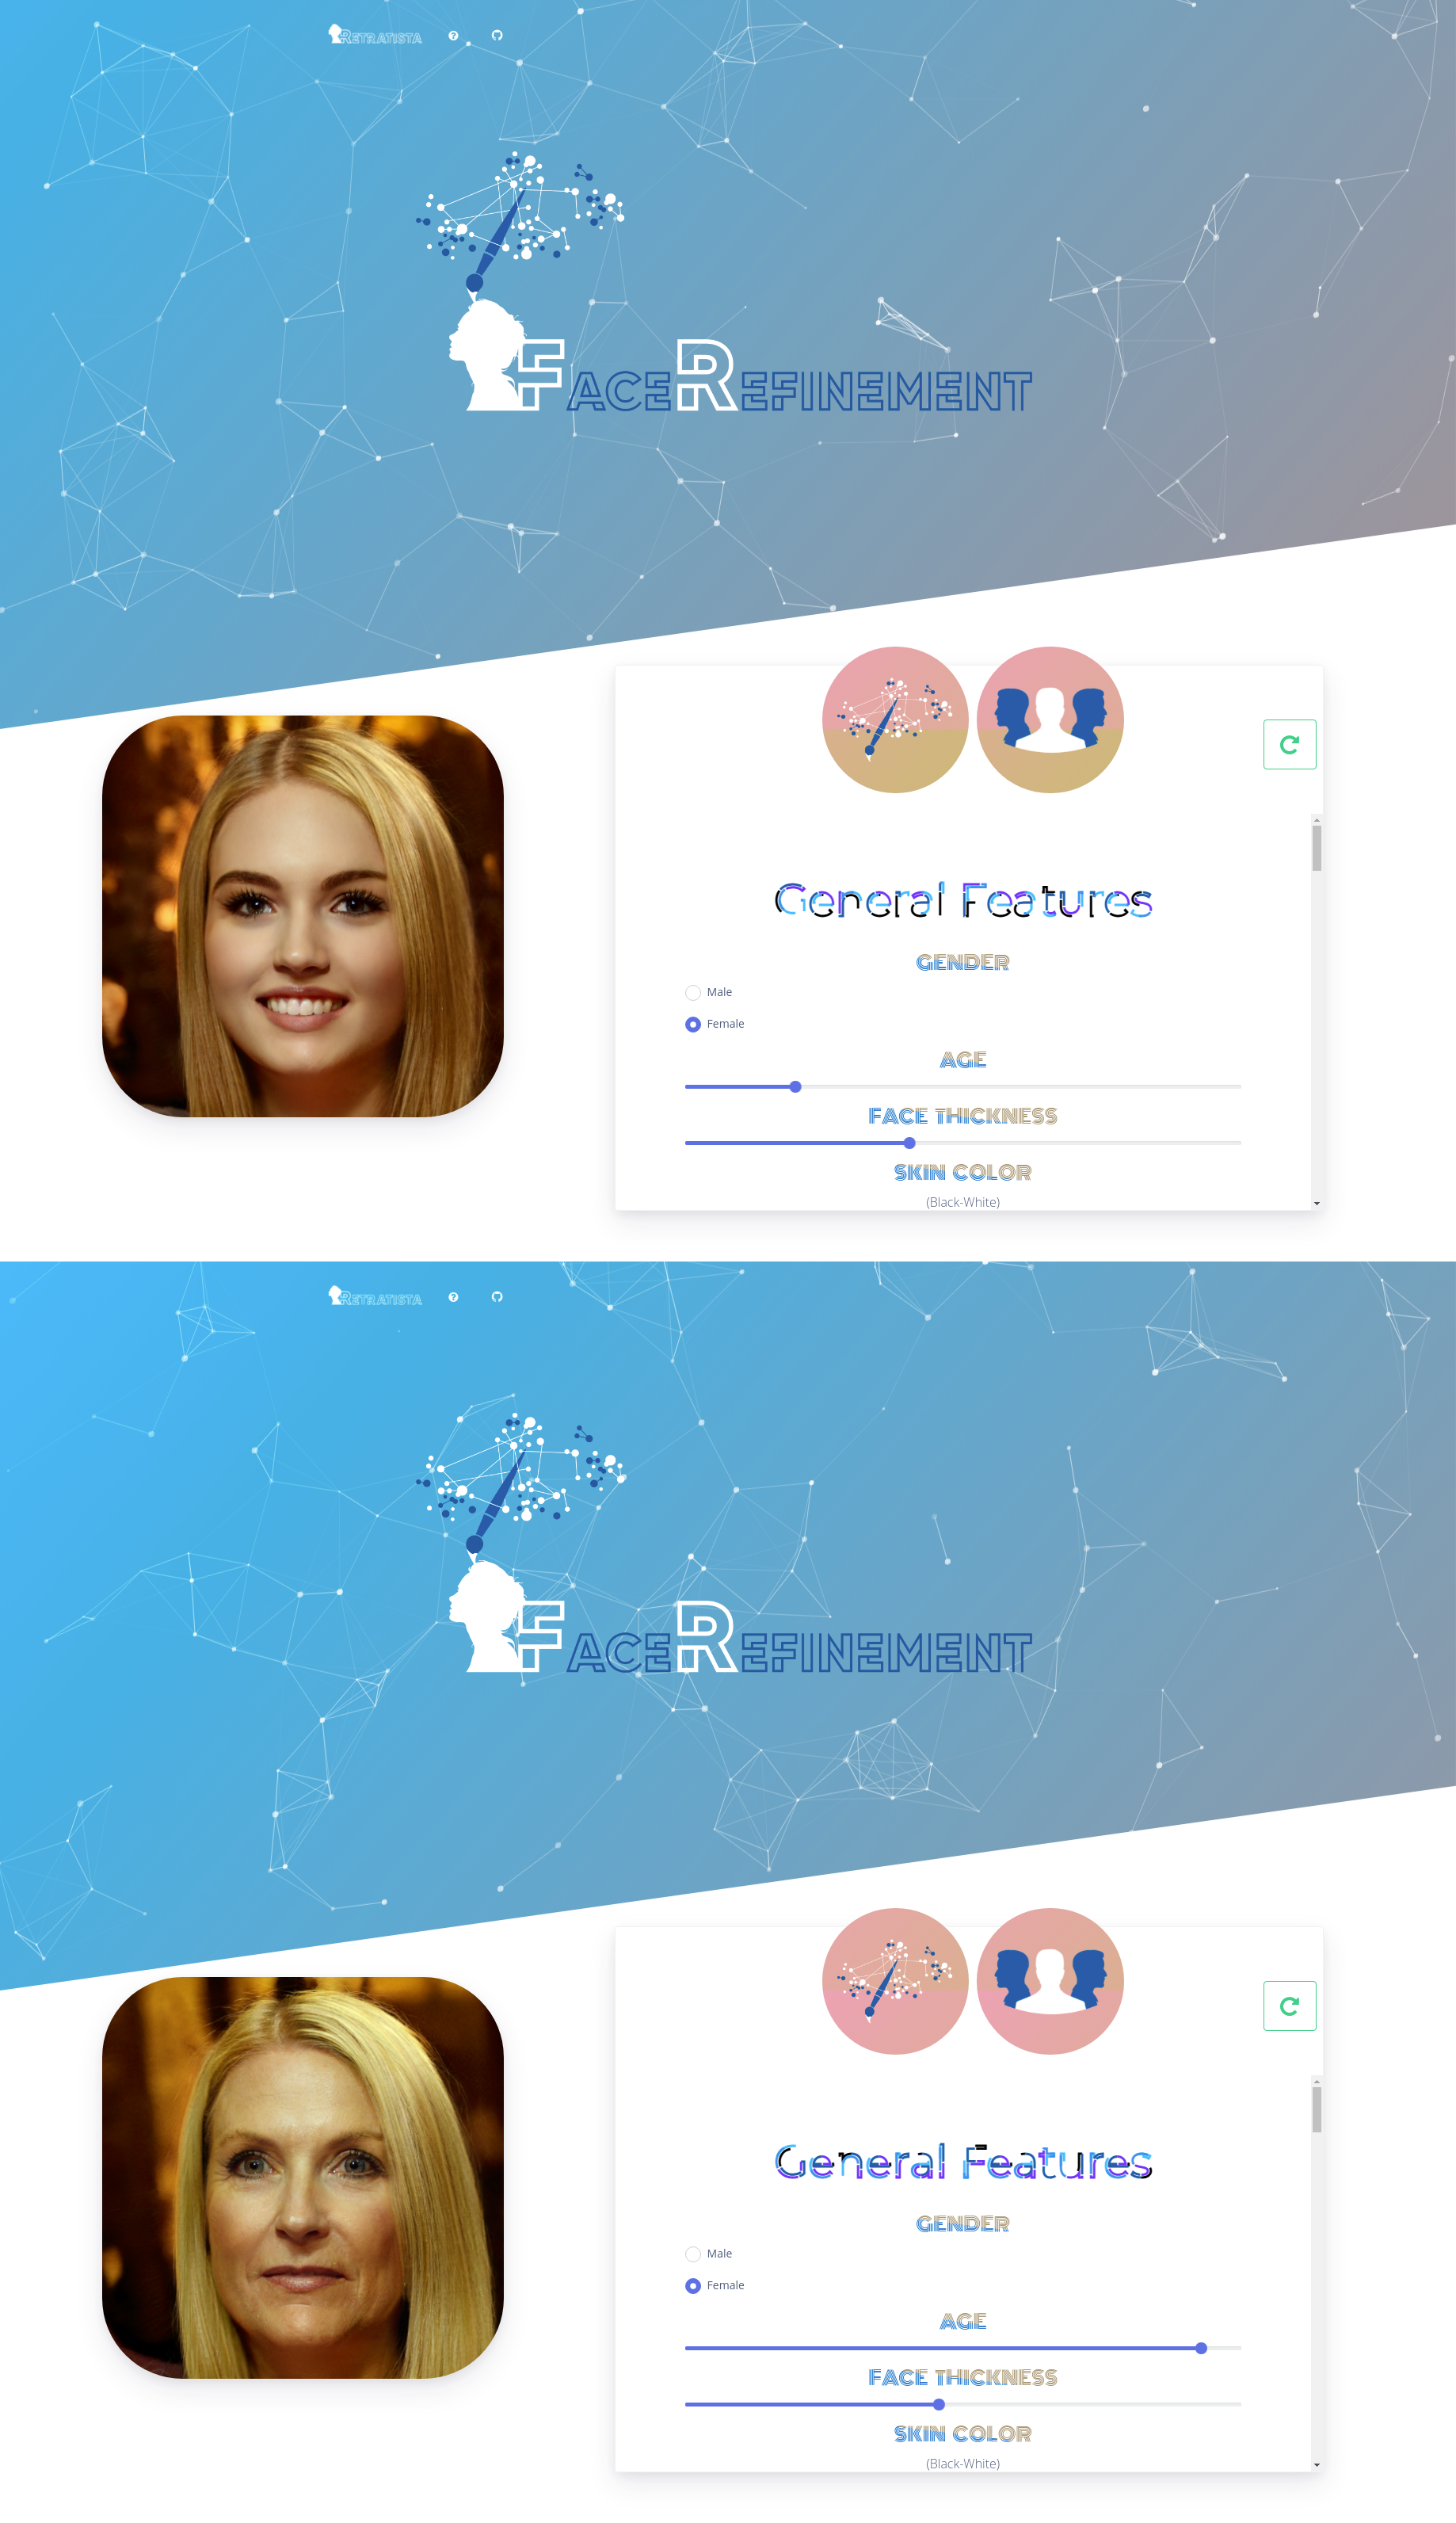
\includegraphics[width=0.7\textwidth]{images/website/refine.png}
    \caption{Refine Page}
    \label{fig:user-refine}
\end{figure}


\subsection{Head Pose Page}
In this page as shown in figure \ref{fig:user-poses}, the user gets 8 different head poses for the same person for extra identification. 

\begin{figure}[H]
    \centering
    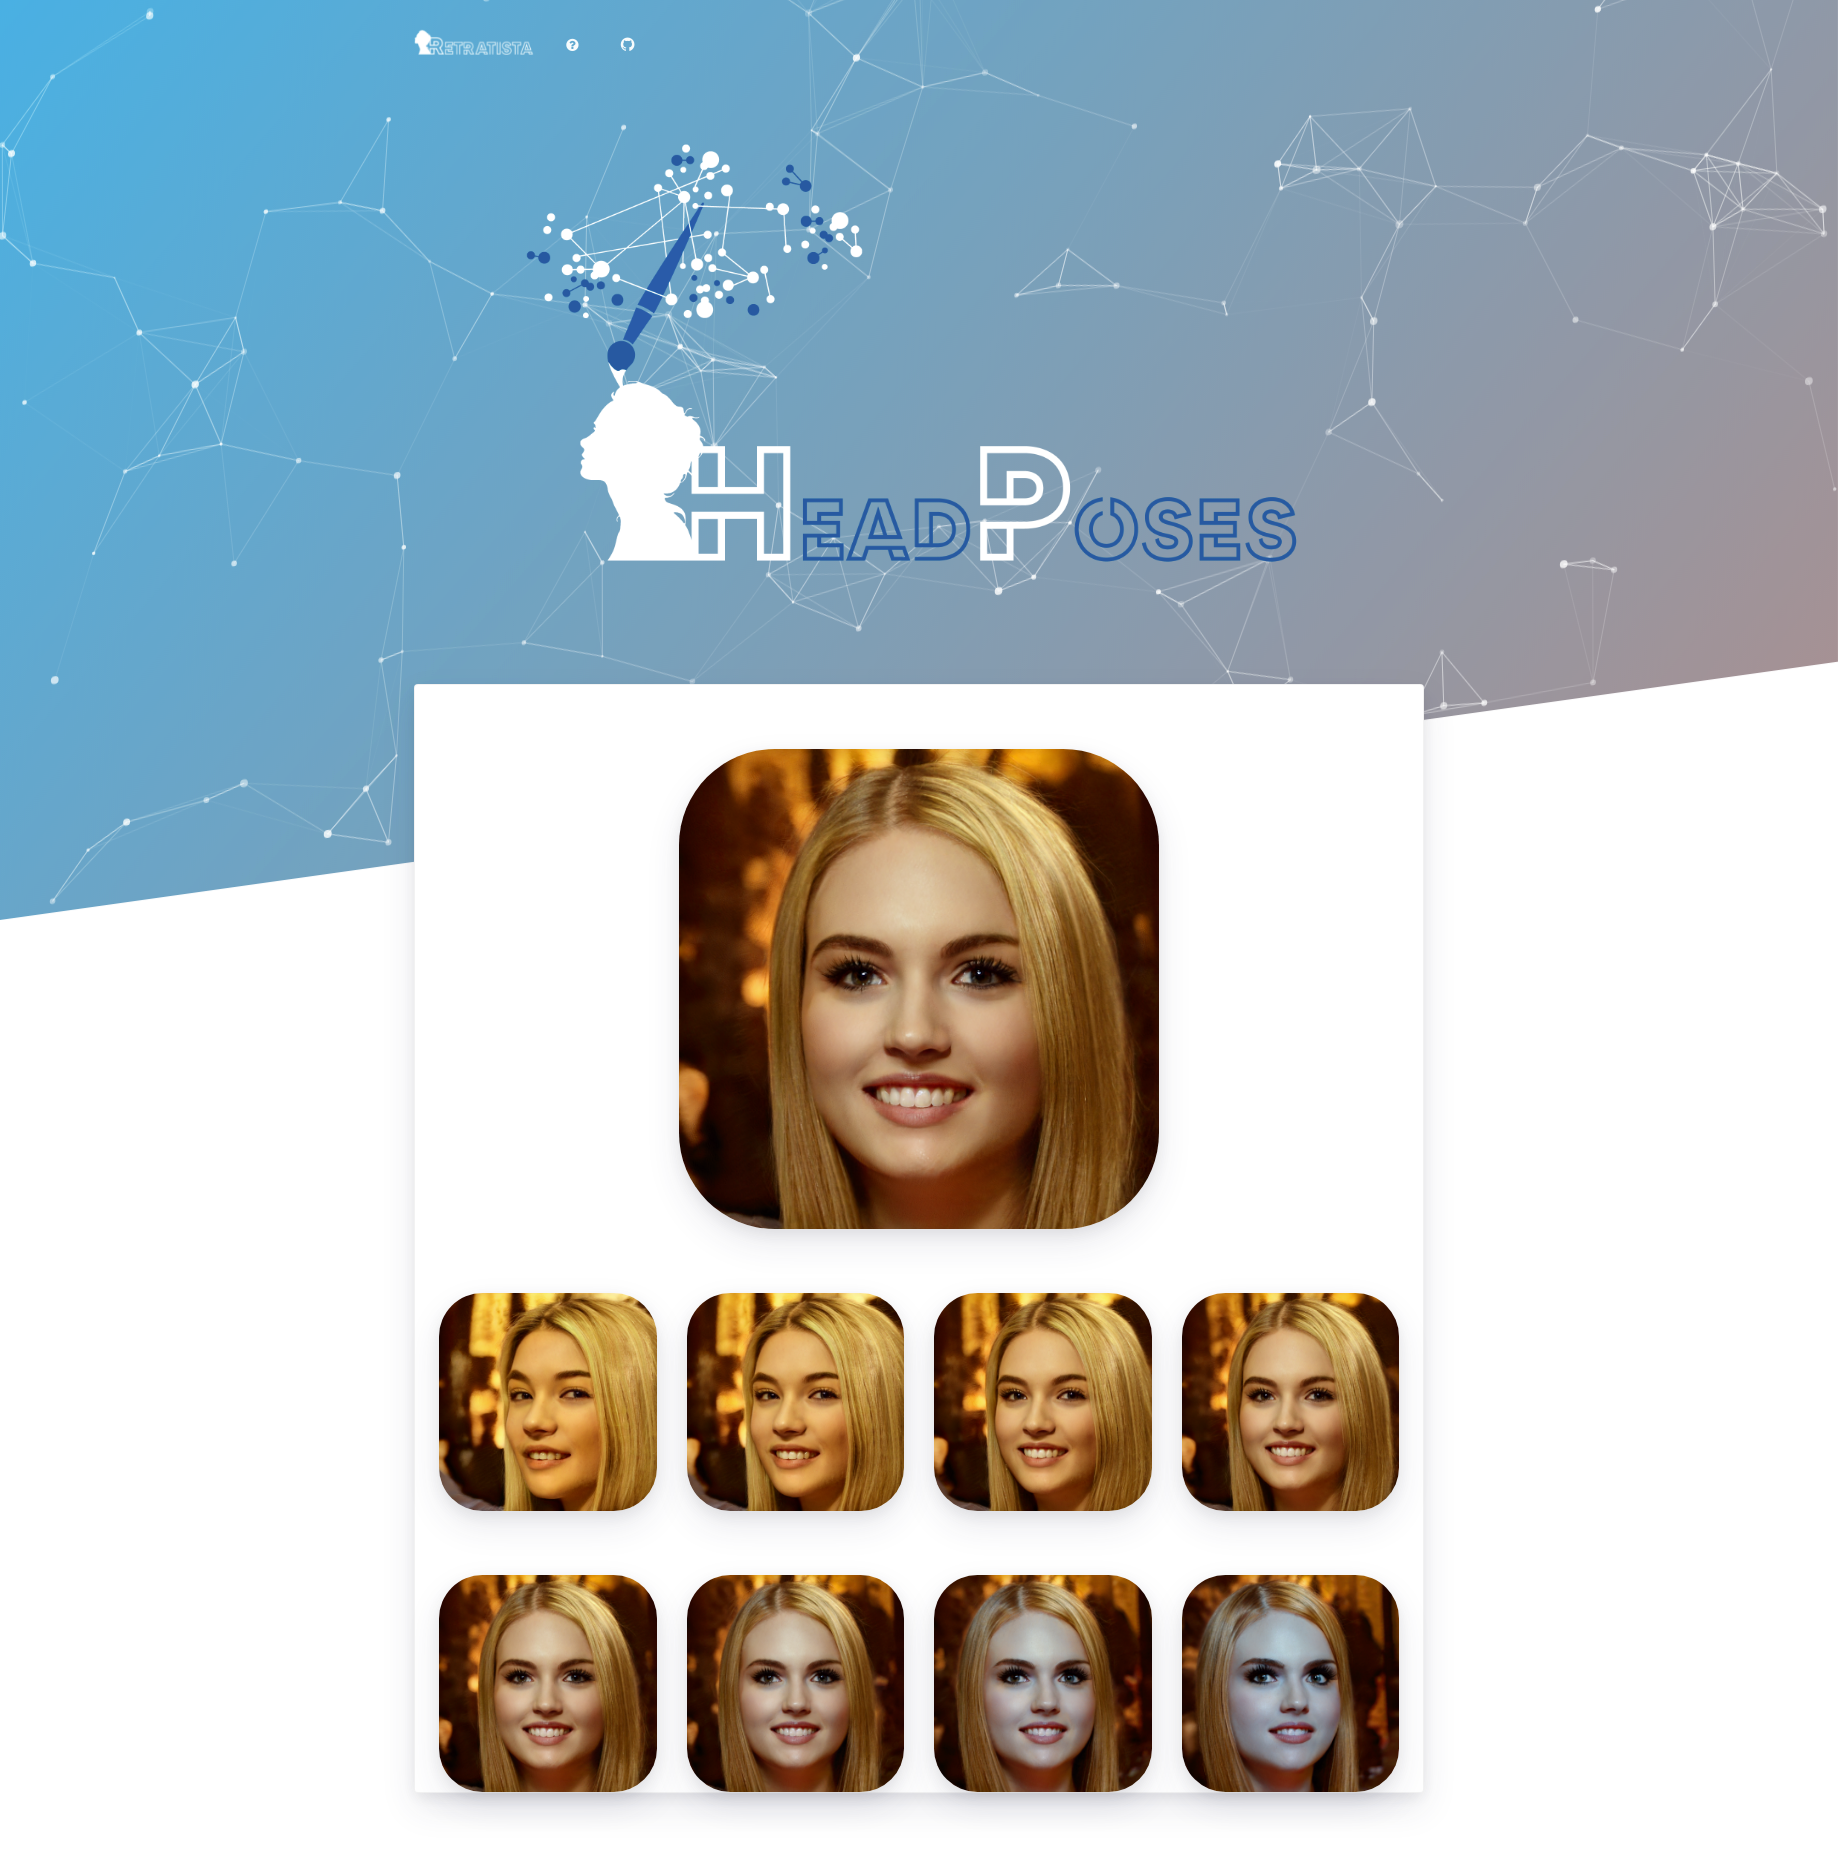
\includegraphics[width=0.9\textwidth]{images/guide/poses.png}
    \caption{Head Pose Page}
    \label{fig:user-poses}
\end{figure}


\subsection{Demo Page}
This Page is a help aid for the user to know how to use the application and to support the user with some extra information about the project, such as
\begin{itemize}
    \item Why is Retratista important?
    \item Statistics
    \item Project Features
    \item How To Use?
    \item Result Samples
    \item Team
\end{itemize}
